\documentclass[9pt, t]{beamer}
\usepackage[ngerman]{babel} 
\usepackage{textgreek}
\usepackage{amsmath}
\usepackage{amssymb}
\usepackage{mathtools}
\usepackage[
backend=biber,
style=alphabetic,
sorting=ynt
]{biblatex}
\bibliography{presentation.bib}
\usepackage{svg}

\usepackage{import}
\import{./}{common.tex}

\usepackage{subcaption}

% Disable navigation buttons
\setbeamertemplate{navigation symbols}{}
\setbeamercovered{transparent}
\newcommand{\margin}{0.05\paperwidth}
\beamersetrightmargin{\margin}
\beamersetleftmargin{\margin}


\title{Approximation von \textpi}
\author{M. van Straten und P. Merz}
\institute{Humboldt-Universität zu Berlin \\
           Sommersemester 2024}
\date{\today}

\usetheme{Berlin}

\begin{document}

\maketitle

\begin{frame}{Inhalt}
    \tableofcontents[pausesections]
\end{frame}

\section{Einführung}

\begin{frame}
    Die Konstante \(\pi\) hat eine natürliche Definition als das Verhältnis
    zwischen dem Umfang und dem Durchmesser eines Kreises.
    \newline\newline
    \textbf{Fundamentaler Bedeutung unter anderem:}
    \begin{itemize}[<+(1)->]
        \item im Gaußschen Integral.
        \item den komplexen Einheitswurzeln.
        \item der Cauchy-Verteilung in der Wahrscheinlichkeitstheorie präsent.
        \item über zahlreiche Disziplinen hinweg.
    \end{itemize}
    \only<6->{
        \(\pi\) ist also eine wichtige Konstanten in der Wissenschaft.
    }
\end{frame}

\begin{frame}{Historie}
    \begin{tabular}{|c||c||c|}
        \hline
        Datum       & Person                          & Korrekte Dezimalstellen \\
        \hline
        ca. 250 v.
        Chr.
                    & Archimedes                      & 2                       \\
        \hline
        1400        & Madhava                         & 10                      \\
        \hline
        1981        & Jean Guilloud                   & 2,000,050               \\
        \hline
        Januar 1988 & \shortstack{Yasumasa Kanada und                           \\ Yoshiaki Tamura} & 201.326.551\\
        \hline
        31.12.2009  & Fabrice Bellard                 & 2,699,999,990,000       \\
        \hline
        14.03.2024  & \shortstack{Jordan Ranous,                                \\
        Kevin O’Brien                                                           \\ und Brian Beeler} & 105,000,000,000,000\\
        \hline
    \end{tabular}
    \cite{Chronology}
\end{frame}

\begin{frame}{Motivation}
    Die Geschichte zeigt: Die genaue Berechnung von \(\pi\) bleibt eine
    mathematische sowie informationstechnische Herausforderung.
    \newline\newline
    \textbf{Ziel dieser Präsentation ist:}
    \begin{itemize}[<+(1)->]
        \item Einführung in mathematische Annäherungsmethoden
        \item \textbf{Analyse in Hinsicht auf:}
              \begin{itemize}[<+(1)->]
                  \item Laufzeit
                  \item Speicherbedarf
                  \item Konvergenzverhalten und Approximationsgenauigkeit
              \end{itemize}
    \end{itemize}
\end{frame}

\section{Theorie}

\subsection{Definitionen}

\begin{frame}{Definitionen}
    \only<1>{%
        \begin{definition}[\(\pi\) in der euklidischen Geometrie]
            Verhältnis zwischen Umfang und Durchmesser eines Kreises
        \end{definition}
        % TODO: cite Analysis I Skript
        Äquivalente Definitionen zum Beispiel in der Analysis über bestimmte
        Nullstellen trigonometrischer Funktionen
    }
    \only<2>{%
        \begin{definition}[Algorithmus]
            % TODO: cite https://de.wikipedia.org/wiki/Algorithmus see citation [1]
            Handlungsvorschrift bestehend aus einer Menge an wohldefinierten
            Schritten
        \end{definition}
        Nützlich, da Algorithmen von Rechnern ausgeführt werden können
    }
    \only<3>{%
        \begin{definition}[Uniforme Teilmenge]
            Eine uniforme Teilmenge \(U\) einer Menge \(M\) ist eine Teilmenge, in der
            jedes Element mit gleicher Wahrscheinlichkeit ausgewählt wird.
            Dies bedeutet, dass für jedes \(x \in M\) die Wahrscheinlichkeit \(P(x \in U)\)
            konstant ist.
        \end{definition}
    }
\end{frame}

\subsection{Annäherungsalgorithmen}

\begin{frame}{Übersicht}
    Es gibt eine große Anzahl an Approximationsalgorithmen für \(\pi\), von
    esoterischen bis hin zu extrem praktikablen.
    \newline\newline
    \textbf{Wir wollen folgende näher betrachten:}
    \begin{itemize}
        \item Monte-Carlo-Simulation
        \item Leibniz-Reihe
        \item Gauß-Legendre-Algorithmus
        \item Chudnovsky-Algorithmus
    \end{itemize}
\end{frame}

\begin{frame}{Monte-Carlo Simulation}
    \begin{minipage}{0.64\textwidth}
        Gegeben der Menge \( \{ (x, y) \mid 0 \le x,y \le 1 \} \eqcolon M \),
        was ist die Wahrscheinlichkeit \( P(M) \), dass ein Punkt in \( M \)
        innerhalb des Einheitskreises liegt?
        \pause
        {%
            \tiny
            \begin{equation*}
                P(M) = \frac{\text{Rote Fläche}}{\text{Gesamte Fläche}}
                = \frac{\pi}{4}
                \pause
                = \frac{\left| \{ (x, y) \in M \mid \sqrt{x^2 + y^2} \le 1 \} \right|}{|M|}
            \end{equation*}
        }
        \pause
        Problem: \( M \) ist überabzählbar\pause, aber für
        \begin{equation*}
            U_1 \subset U_2 \subset \cdots \subset U_n \subset M
        \end{equation*}
        folgt nach dem Gesetz der großen Zahlen, dass
        \begin{equation*}
            \lim_{n \to \infty} P(U_n) = P(M)
        \end{equation*}
        gilt (wenn \( U_n \) eine uniforme Teilmenge von \( M \) ist).
    \end{minipage}
    \begin{minipage}{0.35\textwidth}
        \begin{figure}[H]
            \includesvg[width=\textwidth]{figures/monte-carlo-pi.svg}
        \end{figure}
    \end{minipage}
\end{frame}

\begin{frame}{Leibniz-Reihe}
    Durch Ergebnisse der Analysis leitete Leibniz folgedendes Ergebnis her \cite{Leibniz}
    \[ \pi = \sum_{k=0}^{\infty} \frac{(-1)^k}{2k+1} \]
    \uncover<2->{Annäherung von \(\pi\) über \(n\)-te Partialsumme \(\pi \approx \sum_{k=0}^{n} \frac{(-1)^k}{2k+1}\) }
    \begin{itemize}
        \item<3-> Konvergiert sehr langsam, präzise: Sublineare Konvergenz \\
        \item<3-> Benötigt grob 5 Milliarden Terme um auf 10 korrekte Nachkommastellen zu approximieren
    \end{itemize}
\end{frame}

\begin{frame}{Gauß-Legendre}                                                                                                        %https://web.archive.org/web/20080726033059/http://wwwmaths.anu.edu.au/~brent/pd/rpb028.pdf
    \begin{itemize}
        \item<1-> Approximiert \(\pi\) mittels Folgen, die sich des arithmetischen- und geometrischen Mittels zweier Zahlen bedienen
        \item<2-> \( a_0 = 1 \;\;\; b_0 = \frac{1}{\sqrt{2}} \;\;\; t_0 = \frac{1}{4} \;\;\; p_0 = 1 \)
        \item<3-> \( a_{n+1} = \frac{a_n + b_n}{2} \)
        \item<4-> \( b_{n+1} = \sqrt{a_nb_n} \)
        \item<5-> \( t_{n+1} = t_n - p_n(a_n - a_{n+1})^2 \)
        \item<6-> \( p_{n+1} = 2p_n \)
        \item<7-> \(\pi\) wird dann approximiert durch \[ \pi \approx \frac{(a_{n+1} + b_{n+1})^2}{4t_{n+1}} \]
        \item<8-> Konvergiert quadratisch gegen \(\pi\) \cite{Gauß-Legendre}
    \end{itemize}
\end{frame}

\section{Experimente}

\subsection{Laufzeitanalyse}

\begin{frame}[allowframebreaks]{Laufzeitanalyse}
    \textbf{Was wir experimentell analysieren wollen:}
    \begin{itemize}
        \item Wie lange dauert es, \(n\) Dezimalstellen korrekt zu
              approximieren?
        \item Wie lange dauert es durchschnittlich, eine Dezimalstelle korrekt
              zu approximieren?
    \end{itemize}
    \begin{figure}[H]
        \centering
        \includesvg[width=0.6\textwidth]{figures/runtime-only-slow.svg}
        \caption{Laufzeit, um 7 Dezimalstellen zu approximieren}
    \end{figure}
    \framebreak
    \begin{figure}[H]
        \centering
        \includesvg[width=0.6\textwidth]{figures/runtime-only-fast.svg}
        \caption{Laufzeit, um \(2^{11}\) Dezimalstellen zu approximieren}
    \end{figure}
    \textbf{Fazit:}
    \begin{itemize}
        \item Die Verdoppelung der korrekten Dezimalstellen mit jeder Iteration
              des Gauss-Legendre-Algorithmus wird im Graphen deutlich.
        \item Weniger deutlich aber doch noch zu sehen: der Zuwachs von etwa 14
              Dezimalstellen des Chudnovsky-Algorithmus
        \item Die Leibniz-Reihe benötigt über 10 Sekunden, um 7 Stellen korrekt
              zu approximieren.
        \item Leibniz-Reihe und Monte-Carlo benötigen für jede weitere
              Dezimalstelle exponentiell mehr Zeit.
        \item Der Gauss-Legendre- und der Chudnovsky-Algorithmus laufen in
              polynomialer Zeit.
        \item Die Zeit des Gauss-Legendre-Algorithmus für jede weitere
              Dezimalstelle nimmt ab.
    \end{itemize}
\end{frame}

\subsection{Konvergenz}

\begin{frame}{Daten}
    \begin{figure}
        \begin{center}
            \leavevmode
            \onslide<1>\includegraphics[width=\textwidth]{runtime.png}
            \onslide<2>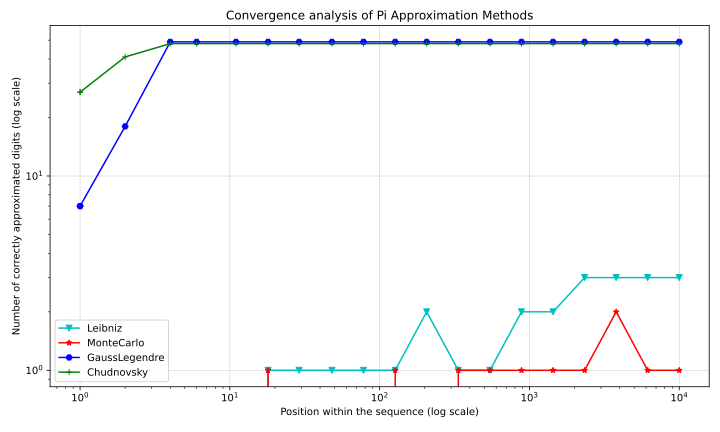
\includegraphics[width=\textwidth]{convergence.png}
        \end{center}
    \end{figure}
\end{frame}

\begin{frame}{Auswertung und Zusammenfassung}

\end{frame}

\subsection{Präzision}

\subsection{Speicherbedarf}

\begin{frame}{Literaturverzeichnis}
    \printbibliography
\end{frame}

\end{document}
